We have shown how the gravitational waves are obtained from the Einstein's field equation. 
By using the transverse traceless gauge we introduced crucial semplifications. 
We want now to explain the important physical consequences of the theoretical results obtained in the previous part.
Throughout the next sections we will use the linearized theory of gravitatinal waves and we consider our metric to be in the TT Gauge.
\subsection{Free particles}
In general relativity the trajectory of a free falling particle is described by the \textbf{geodesic equation}
\begin{equation}
\label{geodesic_eq}
\dv[2]{x^{\beta}}{\tau} + :\Gamma^{\beta} _{\mu \nu}: \,\dv{x^{\mu}}{\tau} \dv{x^{\nu}}{\tau} = 0
\end{equation}
where the coordinates of the particle are represented $x^{\beta}$ and $\tau$ is the proper time.\\
We choose a frame in which a test particle is initially at rest, i.e. with initial four-velocity
\[
u^{\mu} = \dv{x^{\mu}}{\tau} = (1,0,0,0)
\]
We consider a plane wave in the TT gauge propagating towards the test particle. \\
Equation(\ref{geodesic_eq}) can be used to express the initial acceleration of the particle
\[
\qty(
\dv{u^{\beta}}{\tau} 
)_{0}
=
- :\Gamma^{\beta} _{0 0}: 
= -\dfrac{1}{2} \eta ^{\beta \alpha}
\qty(
\partial_{0} h_{\alpha 0} + 
\partial_{0} h_{0 \alpha} + 
\partial_{\alpha} h_{0 0}
)
\]
However, we recall from the TT gauge that
\[
h^{\T}_{0 \alpha} = 0 \qquad  \qquad h^{\T}_{\mu \nu} = \bar{h}^{\T}_{\mu \nu} 
\]
for all $\alpha$. Hence, the initial acceleration of the particle is zero and a free particle, initally at rest, will remain at rest indefinitely.\\
In this constext ''being at rest'' means that the coordinates of the particle do not change, so the TT gauge is a good choice of coordinate. As the gravitational waves propagates, the coordinate system moves with the ripples of the spacetime, in order to keep the particle in the initial position. \\
In the TT gauge free falling bodies are not influenced by  GWs, and their coordinate separation is constant. However, the proper separation is not constant, so let us calculate it.\\
Consider two free falling test particles located at $z=0$ and separated on the x axis by a coordinate distance $L_c$. We still consider a plane wave in the TT gauge propagating in the z direction.\\
The proper distance between the particles is
\bea
L &=& \int _0 ^{L_c} \abs{g_{\mu \nu} \, \dd x^{\mu }\dd x^{\nu }}^{1/2}
=
\int _0 ^{L_c} \sqrt{g_{11}}\dd x = 
\int _0 ^{L_c} \sqrt{1 + h_{+} (t,z=0)} \dd x \\
&\approx &
\int _0 ^{L_c} \qty(1 +\dfrac{1}{2} h_{+} (t,z=0) ) \dd x = L_c \qty(1 + \dfrac{1}{2} h_{+} (t,z=0))
\eea
The proper distance is streched by the passing gravitational wave and the two particles oscillate with a fractional length change given by
\begin{equation}
\dfrac{\delta L}{L} \approx \dfrac{1}{2} h_{+} (t,z=0)
\end{equation}
The proper distance is a very important quantity for a laser interferometer gravitational wave detector, because the phase $\delta \phi$ accumualated by a photon that travels down and back the arm of a laser interferometer is
\[
\delta \phi = \dfrac{4 \pi \delta L}{\lambda}
\]
where $\lambda$ is the wavelength and $\delta L$ is the distance the mirror moves relative to the beam splitter.
Although we used TT gauge to calculate the above formula, it can be shown that this result is gauge independent.\\
If we had considered two particles on the y axis separated by the same coordinate distance, the proper distance would have been
\[
L \approx  L_c \qty(1 - \dfrac{1}{2} h_{+} (t,z=0))
\]
Therefore, recalling the expression of the plus polarization for a plane wave 
$$h_{+} =  A^{\T} _{11} \cos \qty(\omega(t-z))$$ we notice that the particles along x axis are streched, whereas the particles along the y axis are squeezed. 
This is one of the features of the plus polarization, that we will thoroughly analyze in the next section.


\subsection{Geodesic deviation of test particles}
The \textbf{geodesic deviation equation} expresses the relative acceleration between two neighboring geodesics belonging to a one-parameter geodesics $\gamma_s (\tau)$:
\begin{equation}
\label{geudesic_deviation_eq}
\dfrac{D^2}{d \tau ^2} S^{\mu} = :R^{\mu} _{\nu \rho \sigma}: \, T^{\nu} T^{\rho} S^{\sigma}
\end{equation}
 where $S^{\mu} = \partial x^{\mu} / \partial s$ is the deviattion from the geodesic, $T^{\nu} = \partial x^{\mu} / \partial \tau$ is the tangent to the geodesic and the directional covariant derivative is 
\[
\dfrac{D}{d \tau} = \dv{x^{\mu}}{\tau} \, \nabla_{\mu}
\]
The geodesic deviation equation is particularly important because it describes the relative motions of free falling objects and it gives a coordinate-independent measure of the gravitational wave effect. It will also clarify the meaning of the plus and the cross polarizations.\\
If we consider some nearby particles with four-velocities described by a single vector field $u^{\mu}$ and separation vector field $S^{\mu}$, the geodesic deviation equation(\ref{geudesic_deviation_eq}) becomes
\begin{equation}
\dfrac{D^2}{d \tau ^2} S^{\mu} = :R^{\mu} _{\nu \rho \sigma}: \, u^{\nu} u^{\rho} S^{\sigma}
\end{equation}
The four-velocity vector can be approximated with a unit vector in the time direction plus corrections of order $h^{\T} \mu \nu$ and higher, however the Reimann curvature tensor is already first order. Therefore, we ignore the corrections of the four-velocity vector and we write $u^{\nu} =(1,0,0,0)$.\\
Since we have already calculated the Riemann curvature tensor in equation(\ref{reimann_curvature_tensor_first_order}) we recall the result taking into account the TT gauge conditions
\bea
:R^\mu _{00 \sigma }: 
&=&
\dfrac{1}{2} \qty(
\partial_0 \partial_0 :h^{\T \mu} _{\sigma}: -
\partial_0 \partial^\mu h^{\T}_{0 \sigma} -
\partial_\sigma \partial_0 :h^{\T \,\mu} _{ 0}:  +
\partial_\sigma \partial^\mu h_{0 0} ^{\T}
)
\\
&=&
\dfrac{1}{2} \partial_0 \partial_0 :h^{\T \mu} _{\sigma}: \hspace{1.5cm} \text{using } h^{\T} _{\mu 0} =0 
\eea 
In the lowest order approximation the particles are slowly moving, then we have $\tau = x^{0} = t$, so the geodesic deviation equation becomes
\begin{equation}
\pdv[2]{}{t} S^{\mu} = \dfrac{1}{2} S^{\sigma} \pdv[2]{}{t} :h^{\T \mu} _{\sigma}:
\end{equation}
The above equation is a set of differential equations that can be rewritten using the two polarizations of the metric perturbation (equation(\ref{matrix_h_tt}))
\bea
\pdv[2]{}{t} S^{1} &=& \dfrac{1}{2} S^{1} \pdv[2]{}{t} h_{+} + \dfrac{1}{2} S^{2} \pdv[2]{}{t} h_{\times} \\
\pdv[2]{}{t} S^{2} &=& \dfrac{1}{2} S^{1} \pdv[2]{}{t} h_{\times} - \dfrac{1}{2} S^{2} \pdv[2]{}{t} h_{+}
\eea
These can be solved to yield, to lowest order,
\bea
S^{1} = S^{1}(t=0) \qty(1 + \dfrac{1}{2} h_{+})+ \dfrac{1}{2} h_{\times} S^{2}(t=0) \\
S^{2} = S^{2}(t=0) \qty(1 - \dfrac{1}{2} h_{+}) +  \dfrac{1}{2} h_{\times} S^{1}(t=0)
\eea
Let us study the effects of the two polarizations $h_{+}$ and $h_{\times}$ of a gravitational wave, which propagates through the center of a ring of free-falling test particles. 
So, let us use consider a plane wave travelling along the z axis, and let us place a ring of free-falling test particles on the x-y plane  with its center in $(0,0,0)$. 
The ring is initially parametrized by $(\cos \theta, \sin \theta)$ with $\theta \in (0,2\pi]$ and the separation vector $S^{\mu}$ measures the deformation of the ring from its center.\\
Beginning with the case $h_{\times} =0$ and $h_{+} \neq 0$, the solutions of the geodesic deviation equation are
\bea
S^{1} = \cos\theta \qty(1 + \dfrac{1}{2} A^{\T} _{11} \cos (\omega t)) \\
S^{2} = \sin \theta \qty(1 - \dfrac{1}{2} A^{\T} _{11} \cos (\omega t))
\eea
where $h_{+} = A^{\T} _{11} \cos (\omega t)$ for a plane wave. 
The time evolution of the ring is shown in Figure(\ref{plus_polarization}).\\
When the plus polarized gravitational wave propagates through the ring, it increases the proper distance between the ring and its center along the x axis when the phase of the wave is close to $\omega t = 0, 2\pi$, meanwhile it squeezes the test particles along the y axis.
If the phase of the gravitational wave is close to $\omega t = \pi/2, 3\pi/2$ the ring is strecthed along the y axis and the test particles move inwards, therefore, the proper distance from the center of the ring is reduced.
As the wave passes, the test particles bounce back and forth in the shape of $+$ as shown in Figure(\ref{plus_cont}). \\
On the ohter hand, the case where $h_{\times} \neq 0$ and $h_{+} = 0$ yields the geodesic deviation solutions to be
\bea
S^{1} =   \cos \theta + \dfrac{1}{2} \sin \theta A^{\T} _{12} \cos (\omega t) \\
S^{2} = \sin \theta  +  \dfrac{1}{2}  \cos \theta A^{\T} _{12} \cos (\omega t)
\eea
where $h_{\times} = A^{\T} _{12} \cos (\omega t)$ for a plane wave. 
The relationship between these solutions and those for $h_{+} \neq 0$ can be easily found if we consider an angle of $\theta = \pi / 4 $, therefore we obtain
In this case the circle of particles bounce back and forth in the shape of 





\begin{figure}
\centering
    \textbf{ $\mathlarger{\mathlarger{+}}$ Polarization of the gravitational wave}\par\medskip
\makebox[\textwidth][c]{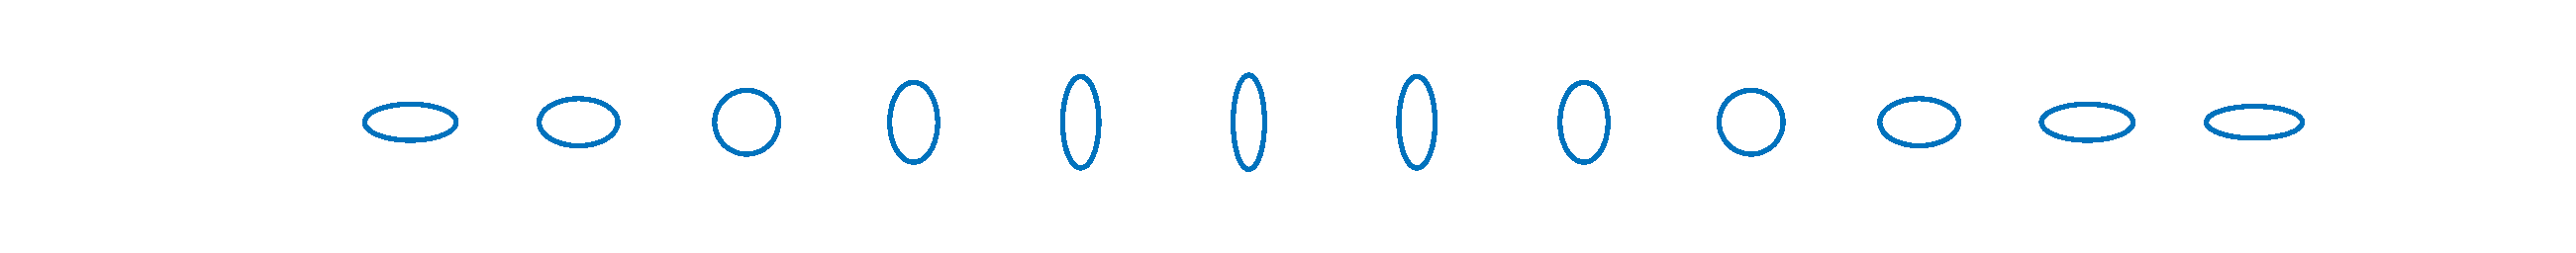
\includegraphics[width=1.3\textwidth]{effects_gw/plus_polarization.eps}}
\caption{Effect of the $h_+$ component on a ring of free-falling test particles at $\omega t = n\pi/6 $ with $n=0,...,12$.}
\label{plus_polarization}
\end{figure}

\begin{figure}
\centering
    \textbf{ $\mathlarger{\mathlarger{\times}}$ Polarization of the gravitational wave}\par\medskip
\makebox[\textwidth][c]{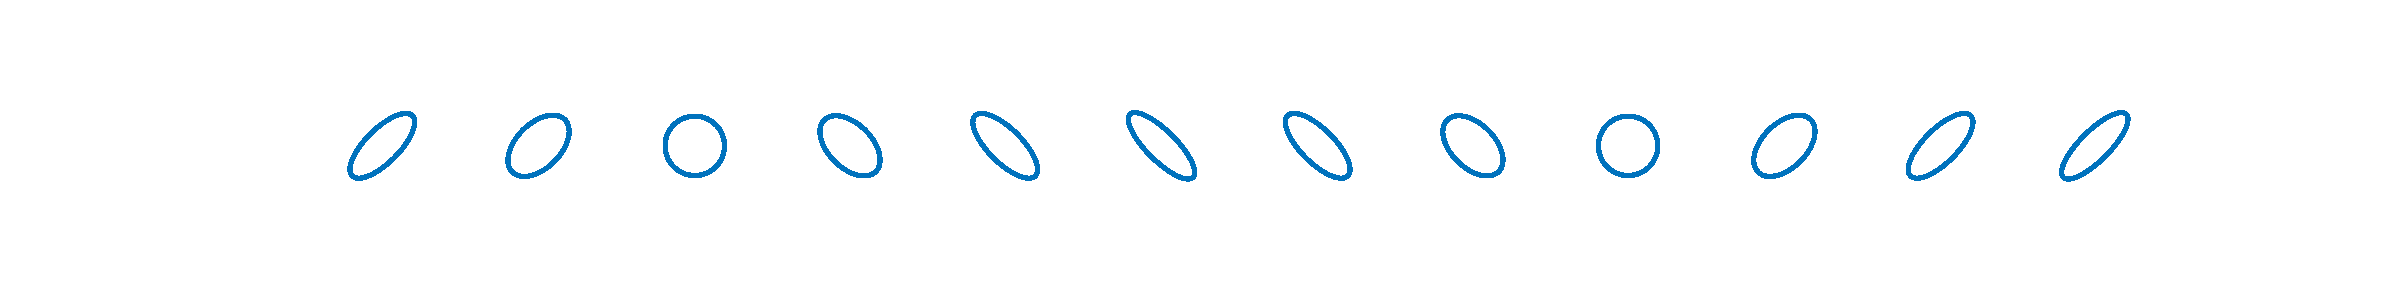
\includegraphics[width=1.3\textwidth]{effects_gw/times_polarization.eps}}
\caption{Effect of the $h_\times$ component on a ring of free-falling test particles at $\omega t = n\pi/6 $ with $n=0,...,12$.}
\end{figure}

\begin{figure}
\centering
    \textbf{ $\mathlarger{\mathlarger{+}}$ Polarization and $\mathlarger{\mathlarger{\times}}$ Polarization}\par\medskip
\centering
\subfloat[][$+$ polarized gravitational wave.]
   {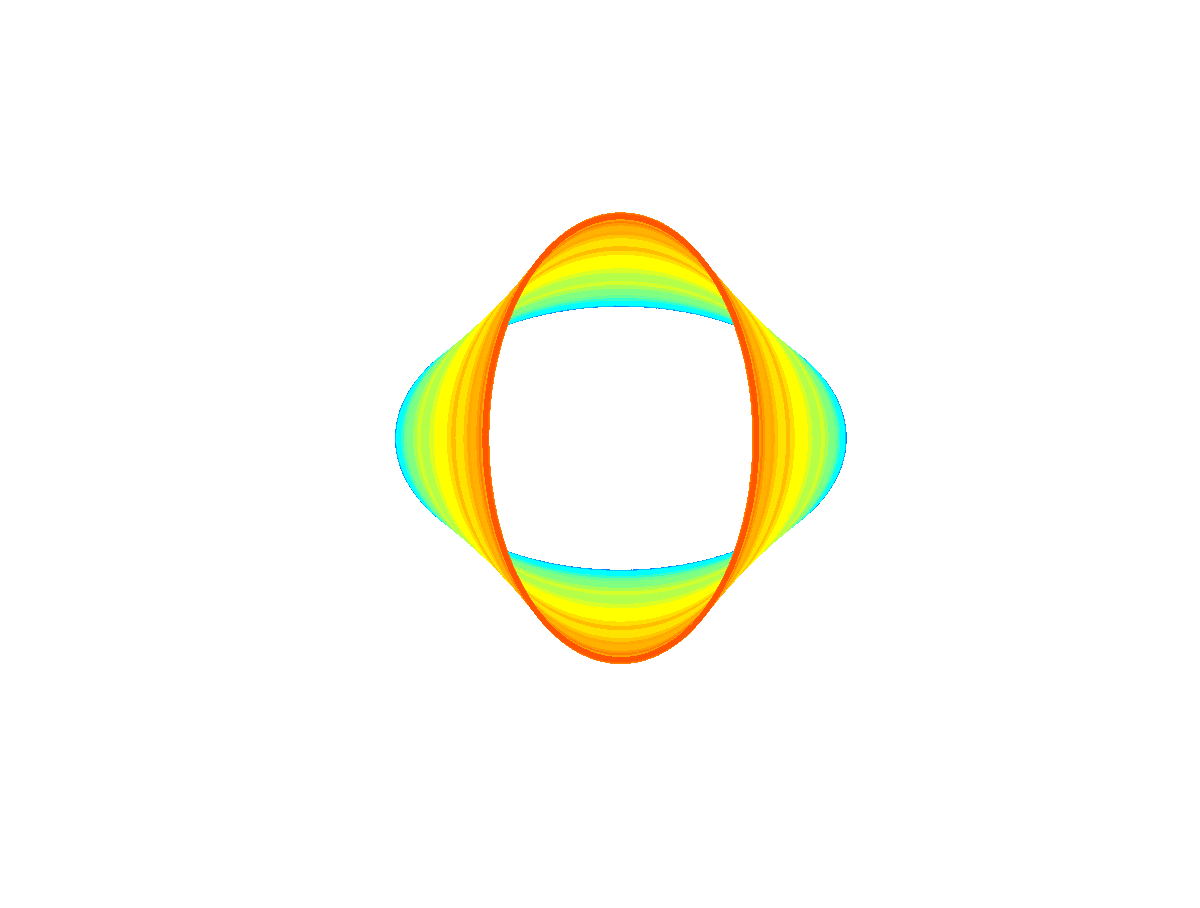
\includegraphics[width=.45\textwidth]{effects_gw/plus_pol_cont.eps}
   \label{plus_cont}} \quad
\subfloat[][$\times$ polarized gravitational wave.]
   {
\includegraphics[width=.45\textwidth]{effects_gw/times_pol_cont.eps}
   \label{times_cont}} \\
\caption{Evolution of a ring of free-falling test particles.}
\label{plus_and_times}
\end{figure}





\subsection{Detection of GW}






